\chapter{Plan de estudios \YYYY}\label{chap:GeneralInfo}

\section{Clasificaci�n de los cursos por niveles}
De acuerdo a la \textit{Computing Curricula}, los cursos son clasificados en 3 niveles: Introductorios (C�digos 100), 
Intermedios  (C�digos 200), Avanzados  (C�digos 300) y orientados a la construcci�n del trabajo de final de carrera  (C�digos 400) tambi�n llamado tesis.

Los cursos de tercer nivel tienen por objetivo abrir varias posibilidades de especializaci�n a trav�s de cursos electivos

Esta propuesta de malla curricular est� basada en el abordaje orientado a objetos. 
El abordaje orientado a la web se escogi� porque hacia eso apuntan las tendencias 
futuras de la computaci�n.

\section{Codificaci�n de los cursos}
Los cursos se encuentran codificados bajo el esquema que se muestra en la Figura~\ref{fig:course-number}:

\begin{figure}[ht]
   \centering
   \includegraphics[width=13cm]{\OutputFigDir/course-coding}
   \caption{Esquema de codificaci�n para los cursos.}
   \label{fig:course-number}
\end{figure}

El tipo de curso esta determinado por sus 2 primeras letras. Los posibles c�digos para estos tipos son:
\input{\OutputTexDir/prefix-description}

Al mismo tiempo, y de acuerdo a la ley universitaria vigente, los cursos est�n clasificados en:
\begin{inparadesc}
\item [AF:] �rea formativa,
\item [AE:] �rea de especialidad,
\item [AB:] �rea b�sica,
\item [AC:] �rea complementaria.
\end{inparadesc}


% Table of courses by semesters
\begin{landscape}
\section{Constituci�n del Plan de Estudios}\label{sec:courses-by-semester}
La relaci�n de cursos se muestra a continuaci�n:
\input{\OutputTexDir/tables-by-semester}

\OnlySPC{Es importante resaltar que todos los semestres podr�an ser completados con cursos extras de acuerdo al perfil de la instituci�n.}
\end{landscape}



% \begin{landscape}
% \section{Distribución de tópicos por curso}\label{sec:topics-by-course}
Las siguientes tablas nos muestran la distribución de todos los tópicos del 
cuerpo del conocimiento de \ac{\currentarea} en todos los cursos.
\section{Distribución de tópicos por curso}\label{sec:topics-by-course}
Las siguientes tablas nos muestran la distribución de todos los tópicos del 
cuerpo del conocimiento de \ac{\currentarea} en todos los cursos.
\section{Distribución de tópicos por curso}\label{sec:topics-by-course}
Las siguientes tablas nos muestran la distribución de todos los tópicos del 
cuerpo del conocimiento de \ac{\currentarea} en todos los cursos.
\input{\OutputTexDir/topics-by-course}
% \end{landscape}

\begin{landscape}
\section{Resultados esperados distribu�dos por curso}\label{sec:outcomes-by-course}
Las siquientes tablas nos muestras una visi�n global de los resultados que se esperan lograr en cada 
curso de la presente malla curricular. 
La lista completa de resultados esperados se encuentra en la Secci�n:~\ref{sec:outcomes}.
\section{Resultados esperados distribu�dos por curso}\label{sec:outcomes-by-course}
Las siquientes tablas nos muestras una visi�n global de los resultados que se esperan lograr en cada 
curso de la presente malla curricular. 
La lista completa de resultados esperados se encuentra en la Secci�n:~\ref{sec:outcomes}.
\section{Resultados esperados distribu�dos por curso}\label{sec:outcomes-by-course}
Las siquientes tablas nos muestras una visi�n global de los resultados que se esperan lograr en cada 
curso de la presente malla curricular. 
La lista completa de resultados esperados se encuentra en la Secci�n:~\ref{sec:outcomes}.
\input{\OutputTexDir/outcomes-by-course}
\end{landscape}

\begin{landscape}
\section{Malla curricular}\label{sec:vision-grafica}
\vspace{-0.3cm}Este documento tambi�n puede ser analizado desde el punto de vista de los prerequisitos de forma gr�fica.
\begin{figure}[h!]
      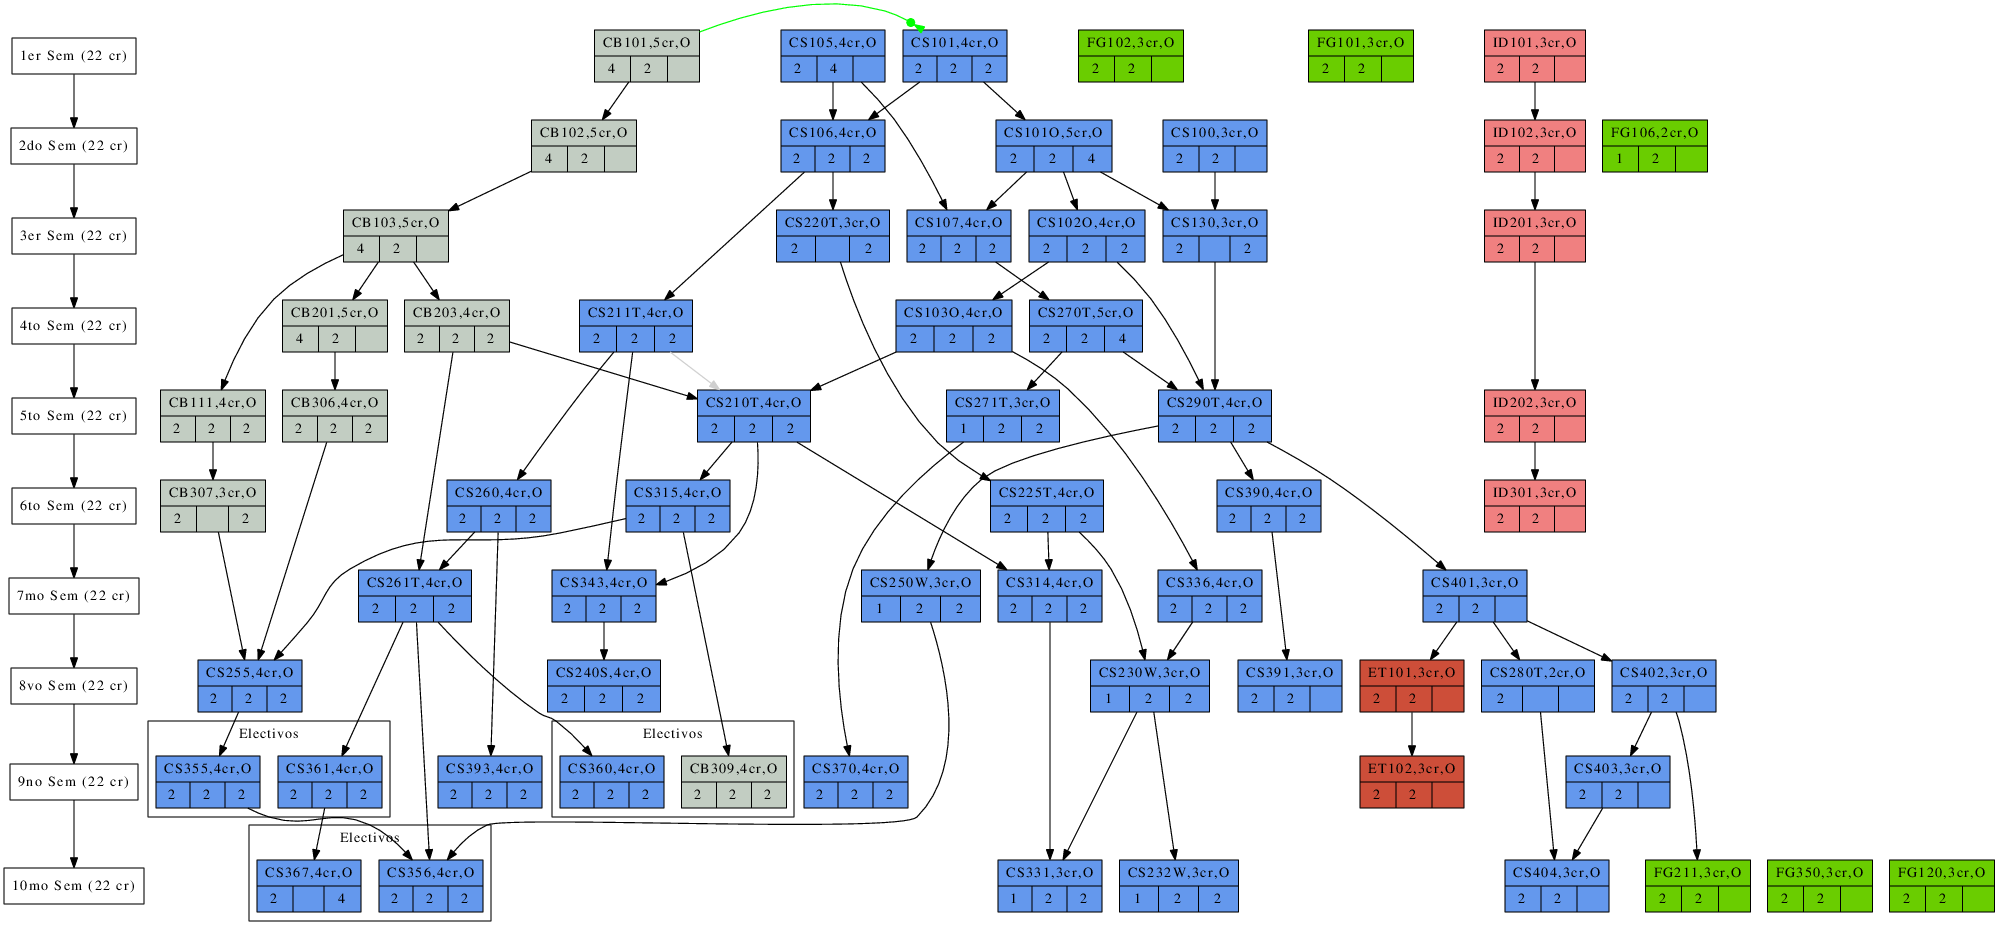
\includegraphics[width=23cm]{\OutputFigDir/small-graph-curricula.ps}
      \label{fig:malla-curricular}
      \caption{Malla curricular \SchoolFullName}
\end{figure}
\end{landscape}

\section{Distribuci�n de cursos en la carrera}
%horas de clase de las mismas
Esta propuesta puede ser analizada por el número de créditos dedicados a cada área
y por niveles de cursos (Introductorios, Intermedios, Avanzados y Proyectos).
\vspace{0.5cm}
 
\begin{figure}[h!]
      \centering
      \includegraphics[width=10cm]{\OutputFigDir/pie-credits}
      \label{fig:pie-credits}
      \caption{Distribución de cursos por áreas considerando creditaje.}
\end{figure}

% \input{\OutputTexDir/distribution-area-by-semester}
\input{\OutputTexDir/distribution-credits-by-area-by-semester}

\begin{figure}[h!]
      \centering
      \includegraphics[width=10cm]{\OutputFigDir/pie-by-levels}
      \label{fig:pie-niveles}
      \caption{Distribución de créditos por niveles de cursos.}
\end{figure} %Graphics by level, by area, etc

% \section{Compatibilidad de la carrera con relaci�n a estandares internacionales}
% En esta secci�n presentamos la distribuci�n de cursos por �reas de concentraci�n en 
% contraste con las propuestas internacionales de las carreras de la \textit{Computing Curricula} 
% de \htmladdnormallink{IEEE-CS}{http://www.computer.org}/\htmladdnormallink{ACM}{http://www.acm.org}.
% 
% Es necesario notar que \underline{en algunos casos las materias podr�an aparecen en m�s de un eje} 
% pues tienen contenido de m�s de una �rea. 
% Por ejemplo, la materia de sistemas operativos contiene unidades de aplicaci�n 
% que pueden ser clasificadas en Tecnolog�a de Informaci�n pero al mismo tiempo contiene fundamentos 
% de como est� estructurado un Sistema Operativo que es del eje de Ciencia de la Computaci�n. 
% En estos casos el creditaje ha sido divido entre los ejes correspondientes.
% \input{\OutputTexDir/list-of-courses-per-area}
% 
% Considerando esta distribuci�n, las figuras \ref{fig:comparing-curves-\currentarea-\currentinstitution-with-CE} 
% a la \ref{fig:comparing-curves-\currentarea-\currentinstitution-with-SE} 
% nos permiten tener una visi�n gr�fica de esta malla curricular frente a las propuestas de 
% carreras presentadas por \htmladdnormallink{IEEE-CS}{http://www.computer.org}/\htmladdnormallink{ACM}{http://www.acm.org} en la \textit{Computing Curricula}
% \input{\OutputTexDir/comparing-with-standards}
